\section{Fundamental groupoid revisited}

Recall the adjunction 
    \begin{tikzcd}
         \Set_{\Delta}
        \arrow[r, shift left, "\tau"]
        &
        \Gpd
        \arrow[l, shift left, "N"]
    \end{tikzcd}
and suppose that $X \in \Set_{\Delta}$ is a Kan complex.

\begin{construction}{Boardman-Vogt Construction}

The homotopy category of $X$ is called $\Ho(X)$ is defined as follows:
\begin{itemize}
    \item 
    $\Ob(\Ho(X))=X_0$
    \item 
    $\hom_{\Ho(X)}(X,Y) = \{f \in X_1 \mid d_1(f)=X , d_0(f)=Y \} / \sim$
\end{itemize}

Recall that a $2$-simplex of $X$
\[
\begin{tikzcd}
    &
    Y
    \arrow[rd,"g"]
    &\\
    X
    \arrow[ru, "f"]
    \arrow[rr,"h"']
    &
    &
    Z
\end{tikzcd} 
\]
should be a "witness" of the fact the $h$ is a composition of $f$ and $g$.
\end{construction}

\begin{problem}
    Why are there different choices of relation $\sim$?
    Given as follows
    \[
    \begin{tikzcd}
        &
        X
        \arrow[rd,"f"]
        &\\
        X
        \arrow[ru, "1_X"]
        \arrow[rr,"g"']
        &
        &
        Y
    \end{tikzcd} 
    = f \sim_1 g
    \qquad
    \begin{tikzcd}
        &
        Y
        \arrow[rd,"1_Y"]
        &\\
        X
        \arrow[ru, "f"]
        \arrow[rr,"g"']
        &
        &
        Y
    \end{tikzcd} 
    = f \sim_2 g
    \]
    \[
    \begin{tikzcd}
        &
        X
        \arrow[rd,"g"]
        &\\
        X
        \arrow[ru, "1_X"]
        \arrow[rr,"f"']
        &
        &
        Y
    \end{tikzcd} 
    = f \sim_3 g
    \qquad
    \begin{tikzcd}
        &
        Y
        \arrow[rd,"1_Y"]
        &\\
        X
        \arrow[ru, "g"]
        \arrow[rr,"f"']
        &
        &
        Y
    \end{tikzcd} 
    = f \sim_4 g
    \]
    where $1_X\coloneqq s_0(X)$. 
    What remains to be shown is that all these are equivalence relations and are in fact the same.
\end{problem}

Lecture 26.11

\begin{prop}
    The four relations above are the same and are equivalence relations.
\end{prop}

\begin{proof}
    We show $(f \sim_3 g \implies f \sim_1 g)$, thus let 
    \[
    \begin{tikzcd}
        &
        X
        \arrow[rd,"g"]
        &\\
        X
        \arrow[ru, "1_X"]
        \arrow[rr,"f"']
        &
        &
        Y
    \end{tikzcd} 
    = \sigma \in X_2
    \]
    We can glue the following $2$-simplices 
    \[
    \begin{tikzcd}
        &
        X
        \arrow[rd,"1_X"]
        &\\
        X
        \arrow[ru, "1_X"]
        \arrow[rr,"1_X"']
        &
        &
        X
    \end{tikzcd} 
    =c^2(X)
    \qquad
    \begin{tikzcd}
        X
        \arrow[rr,"1_X"]
        \arrow[rd,"g"']
        &
        &
        X
        \arrow[ld, "g"]
        \\
        &
        Y
        &
    \end{tikzcd}
    =s_0(g)
    \]
    \[
    \begin{tikzcd}
        X
        \arrow[dd,"f"']
        \arrow[rd,"1_X"]
        &
        \\
        &
        X
        \arrow[ld,"g"]
        \\
        Y
    \end{tikzcd}
    =\sigma
    \]
    to obtain a $3$-horn
    \[
    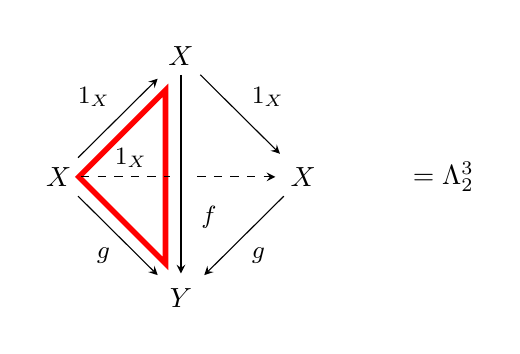
\begin{tikzpicture}[>=stealth,->,shorten >=2pt,looseness=.5,auto]
            \matrix[anchor=center, column sep=1cm, row sep=1cm] at (0,0)
            {
                                & \node(X_1) {$X$};   &                 &\\
             \node(X_0) {$X$};     &                  & \node(X_2) {$X$};& \node(X_24) {$=\Lambda_2^3$};  \\
                                & \node(X_3) {$Y$};   &                 &\\
            };
            \draw[line width=2pt,color=red] (-1.2,1.1) -- (-1.2,-1.1) -- (-2.3, 0) -- cycle;
            \begin{scope}[every node/.style={font=\small\itshape}]
                \draw (X_1) -- node [midway] {$1_X$} (X_2);
                \draw (X_0) -- node [midway] {$1_X$} (X_1);
                \draw (X_0) -- node [midway, swap] {$g$}(X_3);
                \draw [dashed] (X_0) -- node [near start] {$1_X$}(X_2);
                \draw [-,line width=8pt,draw=white]
                (X_1) -- node [pos=0.7] {$f$} (X_3);
                \draw (X_1) -- (X_3);
                \draw (X_2) -- node [midway] {$g$} (X_3);
            \end{scope}
    \end{tikzpicture} 
    \]
    The red $2$-simplex is exactly the one of the equivalence relation $f \sim_1 g$. 
    Since $X$ is an inner Kan complex by assumption, we have the desired horn extension.
    The other direction were part of an exercise and will be included here eventually.
    What remains to be shown, is that it is an equivalence relation.
    \begin{itemize}
        \item 
        (Reflexivity) 
        Let $X \xrightarrow{f} Y$ be in $X_1$, then we have the 2-simplex
        \[
        \begin{tikzcd}
            &
            X
            \arrow[rd,"f"]
            &\\
            X
            \arrow[ru, "1_X"]
            \arrow[rr,"f"']
            &
            &
            Y
        \end{tikzcd} 
        \]
        which means that $\sim$ is associative.
        \item 
        (Symmetry)
        We have the following chain of equivalences
        \[
        f\sim g \iff f\sim_1 g \iff f \sim_3 g \iff g \sim_1f \iff g \sim f
        \]
        \item 
        (Transitivity)
        Let $f\sim g$ and $g \sim h$.
        Consider the following diagrams
        \[
        \begin{tikzcd}
            &
            X
            \arrow[rd, "f"]
            &
            \\
            X
            \arrow[rr, "g"]
            \arrow[ru, "1_X"]
            \arrow[rd, "h"']
            &
            &
            Y
            \arrow[ld,"1_Y"]
            \\
            &
            Y
            &
        \end{tikzcd}
        \qquad
        \begin{tikzcd}
            X
            \arrow[dd, "f"']
            \arrow[rd, "f"]
            \\
            &
            Y
            \arrow[ld, "1_Y"]
            \\
            Y
        \end{tikzcd}
        \] which glued at $1_Y$ and $f$ result in the following horn
        \[
        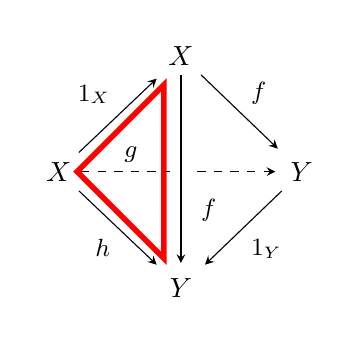
\begin{tikzpicture}[>=stealth,->,shorten >=2pt,looseness=.5,auto]
            \matrix[anchor=center, column sep=1cm, row sep=1cm] at (0,0)
            {
                                & \node(X_1) {$X$};   &                 \\
             \node(X_0) {$X$};     &                  & \node(X_2) {$Y$};  \\
                                & \node(X_3) {$Y$};   &                 \\
            };
            \draw[line width=2pt,color=red] (-0.2,1.1) -- (-0.2,-1.1) -- (-1.3, 0) -- cycle;
            \begin{scope}[every node/.style={font=\small\itshape}]
                \draw (X_1) -- node [midway] {$f$} (X_2);
                \draw (X_0) -- node [midway] {$1_X$} (X_1);
                \draw (X_0) -- node [midway, swap] {$h$}(X_3);
                \draw [dashed] (X_0) -- node [near start] {$g$}(X_2);
                \draw [-,line width=8pt,draw=white]
                (X_1) -- node [pos=0.7] {$f$} (X_3);
                \draw (X_1) -- (X_3);
                \draw (X_2) -- node [midway] {$1_Y$} (X_3);
            \end{scope}
    \end{tikzpicture}
    \]
    By the horn filling property of the inner Kan complex for a 3-horn at position 2 we get the desired $f \sim g$.
    \end{itemize}
\end{proof}

\begin{prop}
    The composition law in $\Ho(X)$ is well defined, unital and associative.
\end{prop}

\begin{proof}
    Suppose that $f \sim f'$. 
    From now on we write $gf \sim h$ to mean that there exists a 2-simplex
    \[
    \begin{tikzcd}
        &
        Y
        \arrow[rd,"g"]
        &\\
        X
        \arrow[ru, "f"]
        \arrow[rr,"h"']
        &
        &
        Z
    \end{tikzcd}   
    \in X_2
    \]
    We prove that if $gf \sim h$, $gf' \sim h'$ and $gf' \sim h$ it follows that $h \sim h'$. 
    So consider the 2-simplices
    \[
    \begin{tikzcd}
        X
        \ar[dd, phantom, shift left=6, "\rho"]
        \ar[dd,"h"']
        \ar[rd,"f"]
        &
        \\
        &
        Y
        \ar[ld,"g"]
        \\
        Z
    \end{tikzcd}
    \qquad
    \begin{tikzcd}
        &
        X
        \ar[rd, "f"]
        &
        \\
        X
        \ar[rr, phantom, shift left=5, "\sigma"]
        \ar[rr, "f'"']
        \ar[ru, "1_X"]
        &&
        Y
    \end{tikzcd}
    \qquad
    \begin{tikzcd}
        X
        \ar[rr, phantom, shift right=5, "\tau"]
        \ar[rr, "f'"]
        \ar[rd, "h'"']
        &&
        Y
        \arrow[ld, "g"]
        \\
        &
        Z
        &        
    \end{tikzcd}
    \]
    which can be glued to obtain a 3-horn
    \[
    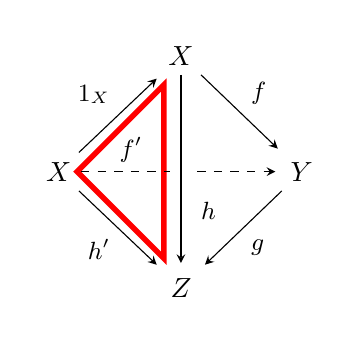
\begin{tikzpicture}[>=stealth,->,shorten >=2pt,looseness=.5,auto]
            \matrix[anchor=center, column sep=1cm, row sep=1cm] at (0,0)
            {
                                & \node(X_1) {$X$};   &                 \\
             \node(X_0) {$X$};     &                  & \node(X_2) {$Y$};  \\
                                & \node(X_3) {$Z$};   &                 \\
            };
            \draw[line width=2pt,color=red] (-0.2,1.1) -- (-0.2,-1.1) -- (-1.3, 0) -- cycle;
            \begin{scope}[every node/.style={font=\small\itshape}]
                \draw (X_1) -- node [midway] {$f$} (X_2);
                \draw (X_0) -- node [midway] {$1_X$} (X_1);
                \draw (X_0) -- node [midway, swap] {$h'$}(X_3);
                \draw [dashed] (X_0) -- node [near start] {$f'$}(X_2);
                \draw [-,line width=8pt,draw=white]
                (X_1) -- node [pos=0.7] {$h$} (X_3);
                \draw (X_1) -- (X_3);
                \draw (X_2) -- node [midway] {$g$} (X_3);
            \end{scope}
    \end{tikzpicture}
    \]
    Now since this is a horn at position $2$ and since $X$ is an inner Kan complex, we obtain a horn extension
    \[
    \begin{tikzcd}
        \Lambda_2^3
        \ar[r, "\gamma"]
        \ar[d]
        &
        X
        \\
        \Delta^3
        \ar[ru, dashed, "\exists \Tilde{\gamma}"']
    \end{tikzcd}
    \] 
    which gives the missing 2-simplex 
    \[
    \begin{tikzcd}
        &
        X
        \ar[rd,"h"]
        &
        \\
        X
        \ar[ru,"1_X"]
        \ar[rr, "h'"]
        &&
        Z
    \end{tikzcd}
    \]
    which yields $h \sim h'$ by the definition of the relation.
    Next we show Unitality, we have 2-simplices
    \[
    \begin{tikzcd}
        &
        X
        \ar[rd,"f"]
        &
        \\
        X
        \ar[ru,"1_X"]
        \ar[rr,"f"']
        &&
        Y
    \end{tikzcd}
    \qquad
    \begin{tikzcd}
        &
        Y
        \ar[rd,"1_Y"]
        &
        \\
        X
        \ar[ru,"f"]
        \ar[rr,"f"']
        &&
        Y
    \end{tikzcd}
    \]
    on equivalence classes this gives $[f] \circ [1_X] =[f] =[1_Y] \circ [f] =[f]$, which exactly means that we have found a unit with respect to the composition.
    Lastly we show Associativity, for that we choose a composition $X \xrightarrow{f} Y \xrightarrow{g} Z \xrightarrow{h} W$.
    \[
    \begin{tikzcd}
        &
        Y
        \ar[rd,"g"]
        &
        \\
        X
        \ar[ru, "f"]
        \ar[rr,"u"]
        \ar[rd, "v"']
        &&
        Z
        \ar[ld,"h"]
        \\
        &
        W    
    \end{tikzcd}
    \]
    which gives the equations 
    \begin{equation}
        [v] = [h] \circ [u] = [h ] \circ ( [g] \circ [f] ).
    \end{equation}
    Now we also have a simplex corresponding to the composition of $g$ and $h$,
    \[
    \begin{tikzcd}
        Y
        \ar[dd,"\alpha"']
        \ar[rd, "g"]
        \\
        &
        Z
        \ar[ld,"h"]
        \\
        W
    \end{tikzcd}
    \]
    putting these three 2-simplices together we obtain a 3-horn.
    \[
    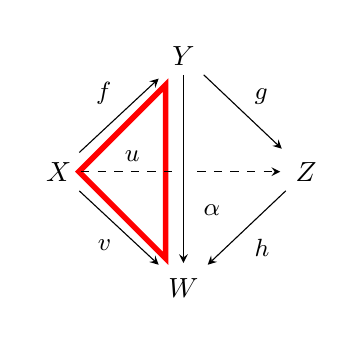
\begin{tikzpicture}[>=stealth,->,shorten >=2pt,looseness=.5,auto]
            \matrix[anchor=center, column sep=1cm, row sep=1cm] at (0,0)
            {
                                & \node(X_1) {$Y$};   &                 \\
             \node(X_0) {$X$};     &                  & \node(X_2) {$Z$};  \\
                                & \node(X_3) {$W$};   &                 \\
            };
            \draw[line width=2pt,color=red] (-0.2,1.1) -- (-0.2,-1.1) -- (-1.3, 0) -- cycle;
            \begin{scope}[every node/.style={font=\small\itshape}]
                \draw (X_1) -- node [midway] {$g$} (X_2);
                \draw (X_0) -- node [midway] {$f$} (X_1);
                \draw (X_0) -- node [midway, swap] {$v$}(X_3);
                \draw [dashed] (X_0) -- node [near start] {$u$}(X_2);
                \draw [-,line width=8pt,draw=white]
                (X_1) -- node [pos=0.7] {$\alpha$} (X_3);
                \draw (X_1) -- (X_3);
                \draw (X_2) -- node [midway] {$h$} (X_3);
            \end{scope}
    \end{tikzpicture}
    \]
    Now the missing simplex corresponds to 
    \begin{equation}
        [v] = [ \alpha ] \circ [f] =( [h] \circ [g]) \circ [f],
    \end{equation}
    since $X$ is an inner Kan complex, the horn can be filled and we obtain associativity by combining equations $(1)$ and $(2)$.
\end{proof}

\begin{rmk}
    The result, that $\Ho(X)$ is a well defined category is known as Joyal's coherence lemma.
\end{rmk}

\begin{prop}
    Let $X \in \SetD$ be a Kan complex, then $\Ho (X)$ is a groupoid.
\end{prop}

\begin{proof}
    Let $f \in \Ho(X)$ be a morphism. 
    Then we have a simplex
    \[
    \begin{tikzcd}
        & 
        X
        \arrow[rd, "f"]
        &
        \\
        Y
        \arrow[rr, "1_Y"']
        \arrow[ru, dashed, "\exists g"]
        &&
        Y
    \end{tikzcd}
    \]
    which corresponds to $[g] \circ [f] = [1_Y]$.
\end{proof}

\begin{cor}
    Let $X \in \SetD$ be a Kan complex, then $L \Ho(X) \cong \Ho(X)$.
\end{cor}

\begin{proof}
     Consider the adjunction 
     \[
     \begin{tikzcd}
        \Cat
        \arrow[r, shift left, "L"]
        &
        \Gpd 
        \arrow[l, shift left, "j"]
    \end{tikzcd}
     \]
     where $j$ is just the inclusion. 
     Then the counit $\epsilon$ of the adjunction is the desired isomorphism, since $L\Ho(X)$ actually means $jL\Ho(X)$, that is considering $L \Ho(X)$ as a category not a groupoid.
\end{proof}

\begin{prop}
    Let $X \in \SetD$ be an inner Kan complex, then $\Ho(X) \cong \tau X$, where $\tau$ is the right adjoint of the nerve functor.
\end{prop}

\begin{proof}
    Let $\mathcal{D} \in \Cat$, since $N(\mathcal{D}) \in \SetD$ is $2$-coskeletal, we have a natural bijection:
    \[
    \Hom_{\SetD}(X, N( \mathcal{D})) \isomorphism \Hom_{\SetD}(\tru_2X,\tru_2(N(\mathcal{D}))
    \]
    Consider a morphism $\tru_2(X) \xrightarrow{f} \tru_2(N(\mathcal{D}))$ given by
    \[
    \begin{tikzcd}
        \tru_2
        \arrow[d,"f"]
        &
        X\colon \dotsc 
        &
        X_2
        \arrow[r, altstackar=5]
        \arrow[d,"f_2"]
        &
        X_1
        \arrow[r,altstackar=3]
        \arrow[d,"f_1"]
        &
        X_0=\Ob(\Ho(X))
        \arrow[d,"f_0"]
        \\
        \tru_2(N(\mathcal{D}))
        &
        N(\mathcal{D})\colon \dotsc 
        &
        N(\mathcal{D})_2
        \arrow[r, altstackar=5]
        &
        N(\mathcal{D})_1
        \arrow[r,altstackar=3]
        &
        N(\mathcal{D})_0=\Ob(\mathcal{D})
    \end{tikzcd}
    \]
    Note that $N(\mathcal{D})_1=\Mor( \mathcal{D} )$.
    We have for any $\alpha \in X_1$ that $f_0(d_0(\alpha)) = \text{target} (f_1(\alpha))$ and that for any $d_1(\alpha) \xrightarrow{\alpha}d_0(\alpha)$ that $f_0(d_1(\alpha))= \text{source}(\alpha)$.
    Now for 2-simplices we have
    \[
    \alpha \sim \beta
     \begin{tikzcd}
        &
        x
        \arrow[rd,"\alpha"]
        &\\
        x
        \arrow[ru, "1_x"]
        \arrow[rr,"\beta"']
        &
        &
        y
    \end{tikzcd}   
    \xmapsto{f_2}
    \begin{tikzcd}
        &
        f_0(x)
        \arrow[rd,"f_1(\alpha)"]
        &\\
        f_0(x)
        \arrow[ru, "\id_{f_0(x)}"]
        \arrow[rr,"f_1(\beta)"']
        &
        &
        f_0(y)
    \end{tikzcd}
    \]
    Thus $f_1(\alpha)=f_1(\beta)$ which results in 
    \[
    \Hom_{\Set_{\Delta}}(\tru_2(X), \tru_2(N(\mathcal{D})) \isomorphism \Hom_{\Cat}(\Ho(X), \mathcal{D})
    \]
\end{proof}

\begin{cor}
    Let $X \in \Set_{\Delta}$ be a Kan complex. 
    Then $\pi_1(X)=\Ho(X)$ and for all $x \in X_0$ it holds that
    $\pi_1(X,x) \isomorphism \Hom_{\Ho(X)}(X,X)$.
\end{cor}

\begin{proof}
    We know that 
    \[
    \pi_1(X,x) = \Hom_{\pi_1(X)}(x,x) \isomorphism \Hom_{\Ho(X)}(x,x)
    \]
    as well as 
    \[
    \pi_1(X)=L(\tau X) \isomorphism L(\Ho(X)) \isomorphism \Ho(X).
    \]
    by putting the previous two corollaries together.
\end{proof}

\subsection{Exercises}

\begin{Exercise}
    Fix an inner Kan complex $ X $. For edges $ f , g , h \in X_1 $ we say $ g \cdot f \sim h $ if there exists a 2 simplex such that $d_0 ( \sigma ) = g , d_1 ( \sigma ) = h $ and $ d_2 ( \sigma ) = f $.
    
    \begin{enumerate}
        \item 
        Show Joyal's Coherence Lemma:
    
        Consider $ \alpha: \bold{sk}_1 ( \Delta^3 ) \to X $ with $ \alpha_1 ( f_{21} ) \cdot \alpha_1 ( f_{10} ) \sim \alpha_1 ( f_{20} ) $ and $ \alpha_1 ( f_{32} ) \cdot \alpha_1 ( f_{21} ) \sim \alpha_1 ( f_{31} )$.
        Then $ \alpha_1 ( f_{31} ) \cdot \alpha_1 ( f_{10} ) \sim \alpha_1 ( f_{30} )$ if and only if $ \alpha_1 ( f_{32} ) \cdot \alpha_1 ( f_{20} ) \sim \alpha_1 ( f_{30} ) $.
        Here we denote by $ f_{ji} $ the unique morphism $ f_{ i , j } : [1 ] \to [ 3 ]$ with image $ \{ i < j \} \subseteq [ 3 ] $.
    \end{enumerate}
    
    We define the following four relations on $X_1$.
    
    \begin{align*}
        f \sim_1 g & \iff f \cdot s_0 ( d_1 ( f ) ) \sim g 
        \\
        f \sim_3 g & \iff g \cdot s_0 ( d_1 ( g ) ) \sim f
    \end{align*}
    \qquad
    \begin{align*}
        f \sim_2 g & \iff f \cdot s_0 ( d_0 ( f ) ) \sim g 
        \\
        f \sim_4 g & \iff g \cdot s_0 ( d_0 ( g ) ) \sim f
    \end{align*}
    
    \begin{enumerate}[label=(\alph*), resume]
        \item 
        Show that $ f \sim_1 g \iff f \sim_2 g $ and that $ f \sim_1 g \implies f \sim_3 g $.
    
        \item 
        Deduce that all four relations agree.
    
        \item 
        Conclude that the relation $ \simeq \coloneqq \sim_1 $ is an equivalence relation on $X_1$.
    \end{enumerate}
\end{Exercise}

\begin{Exercise}
    Show that the homotopy category $ \Ho ( N ( \mathcal{ C } ) ) $ of the nerve of a small category $ \mathcal{ C } $ is isomorphic to $ \mathcal{ C } $.
\end{Exercise}

\begin{Exercise}
    Let $ G $ be a simplicial group.
    Let $ n \in \mathbb{ N }_+ $ and $ 0 < l < n+1 $. 
    For $ y \in G_{n+1} $ we say $ x \in G_n $ is $l$-compatible if $ d_i ( x ) = d_l ( d_{i+1} ( y ) ) $ if $ l \leq i $. 
    Moreover, we say $x$ is $ ( k , l ) $-compatible for $ 0 \leq k < l $ if additionally $ d_i ( x ) = d_{ l-1 } ( d_i ( y ) ) $ for $ 0 \leq i < k $.
    
    \begin{enumerate}[label=(\alph*)]
        \item 
        Show that if $ x $ is $ ( k , l ) $-compatible with $ y \in G_{n+1} $, then we have for $ y' \coloneqq s_{l-1} ( x \cdot ( d_l ( y ))^{-1} ) \cdot y  \in G_{n+1} $ that 
        \[
        d_i ( y' ) =
        \begin{cases} 
            d_i(y) &\text{ if } k < l
            \\
            x &\text{ if } i = l 
            \\
            d_i ( y ) &\text{ if } i > l
        \end{cases}
        \]
    
        \item 
        Give the notion of cocompatibility which is dual to compatibility.
    
        \item 
        Show that the underlying simplicial set of $ G $ is a Kan complex.
        
    \end{enumerate}
\end{Exercise}

\begin{Exercise}
    Recall from Exercise 6.2 the definition of the $n$-coskeleton of a simplicial set $ X $ and $ n \in \mathbb{N}_0 $.
    
    \begin{enumerate}[label=(\alph*)]
        \item 
        Show that if $ X $ is $n$-coskeletal, then for any $ m > n $ we have an isomorphism
        \[
            \Hom_{\SetD}( \Delta^m , X ) 
            \to 
            \Hom_{\SetD} ( \partial \Delta^m , X ) 
        \]
        induced by the inclusion $ \partial \Delta^m \subseteq \Delta^m$.
    
        \item 
        Show that if for some $ m \in \mathbb{N}_+$ the inclusion $ \partial \Delta^m \subseteq \Delta^m $ induces an isomorphism for $ X $ as above, then for any morphism $ Y \to X $ of simplicial sets, the component $ f_m \colon Y_m \to X_m $ is completely determined by $ \tru_{m-1} ( f ) $.
    
        \item 
        Conclude that a simplicial set $ X $ is $ n $-coskeletal if and only if for every $ m > n $ the inclusion $ \partial \Delta^m \subseteq \Delta^m $ induces an isomorphism $ \Hom_{ \SetD } ( \Delta^m , X ) \to \Hom_{\SetD} ( \partial \Delta^m , X )$.
        
    \end{enumerate}
\end{Exercise}
